\documentclass{article}
\usepackage{multicol}
\usepackage{graphicx}
\graphicspath{ {images/} }

\title{Catalina Tiles}
\author{Matthew Gallant}
\date{September 26, 2015}

\begin{document}
\maketitle

\begin{center}
\includegraphics[width=\linewidth]{catalina_tiles}
\end{center}

\section{Introduction}
Catalina Tiles was created for the exercise ``Luck Tac Toe'' in Chapter 5 of \textit{Challenges for Game Designers} by Brenda Brathwaite \& Ian Schreiber. The challenge given was to ``modify [Tic-Tac-Toe] by adding one or more chance-based mechanics''. The game should also be ``good for adult players''.

\section{Materials}
\begin{itemize}
  \item Four 4-sided dice
  \item 40 red tokens and 40 blue tokens
  \item Board with nested 3x3 grid (see diagram on page 2)
\end{itemize}

\section{Rules}
The game is played on a nested 3x3 grid; each tile in the large 3x3 grid contains a small 3x3 grid within it.

Players take turns claiming a tile in one of the small grids (see ``Claiming'' below). One player claims tiles by placing red tokens, the other uses blue tokens. The oldest player plays first.

A player who claims 3 tiles in a row within a single small grid (horizontally, vertically or diagonally) claims that tile in the large grid.

A player who claims 3 large tiles in a row wins the game.

\begin{center}
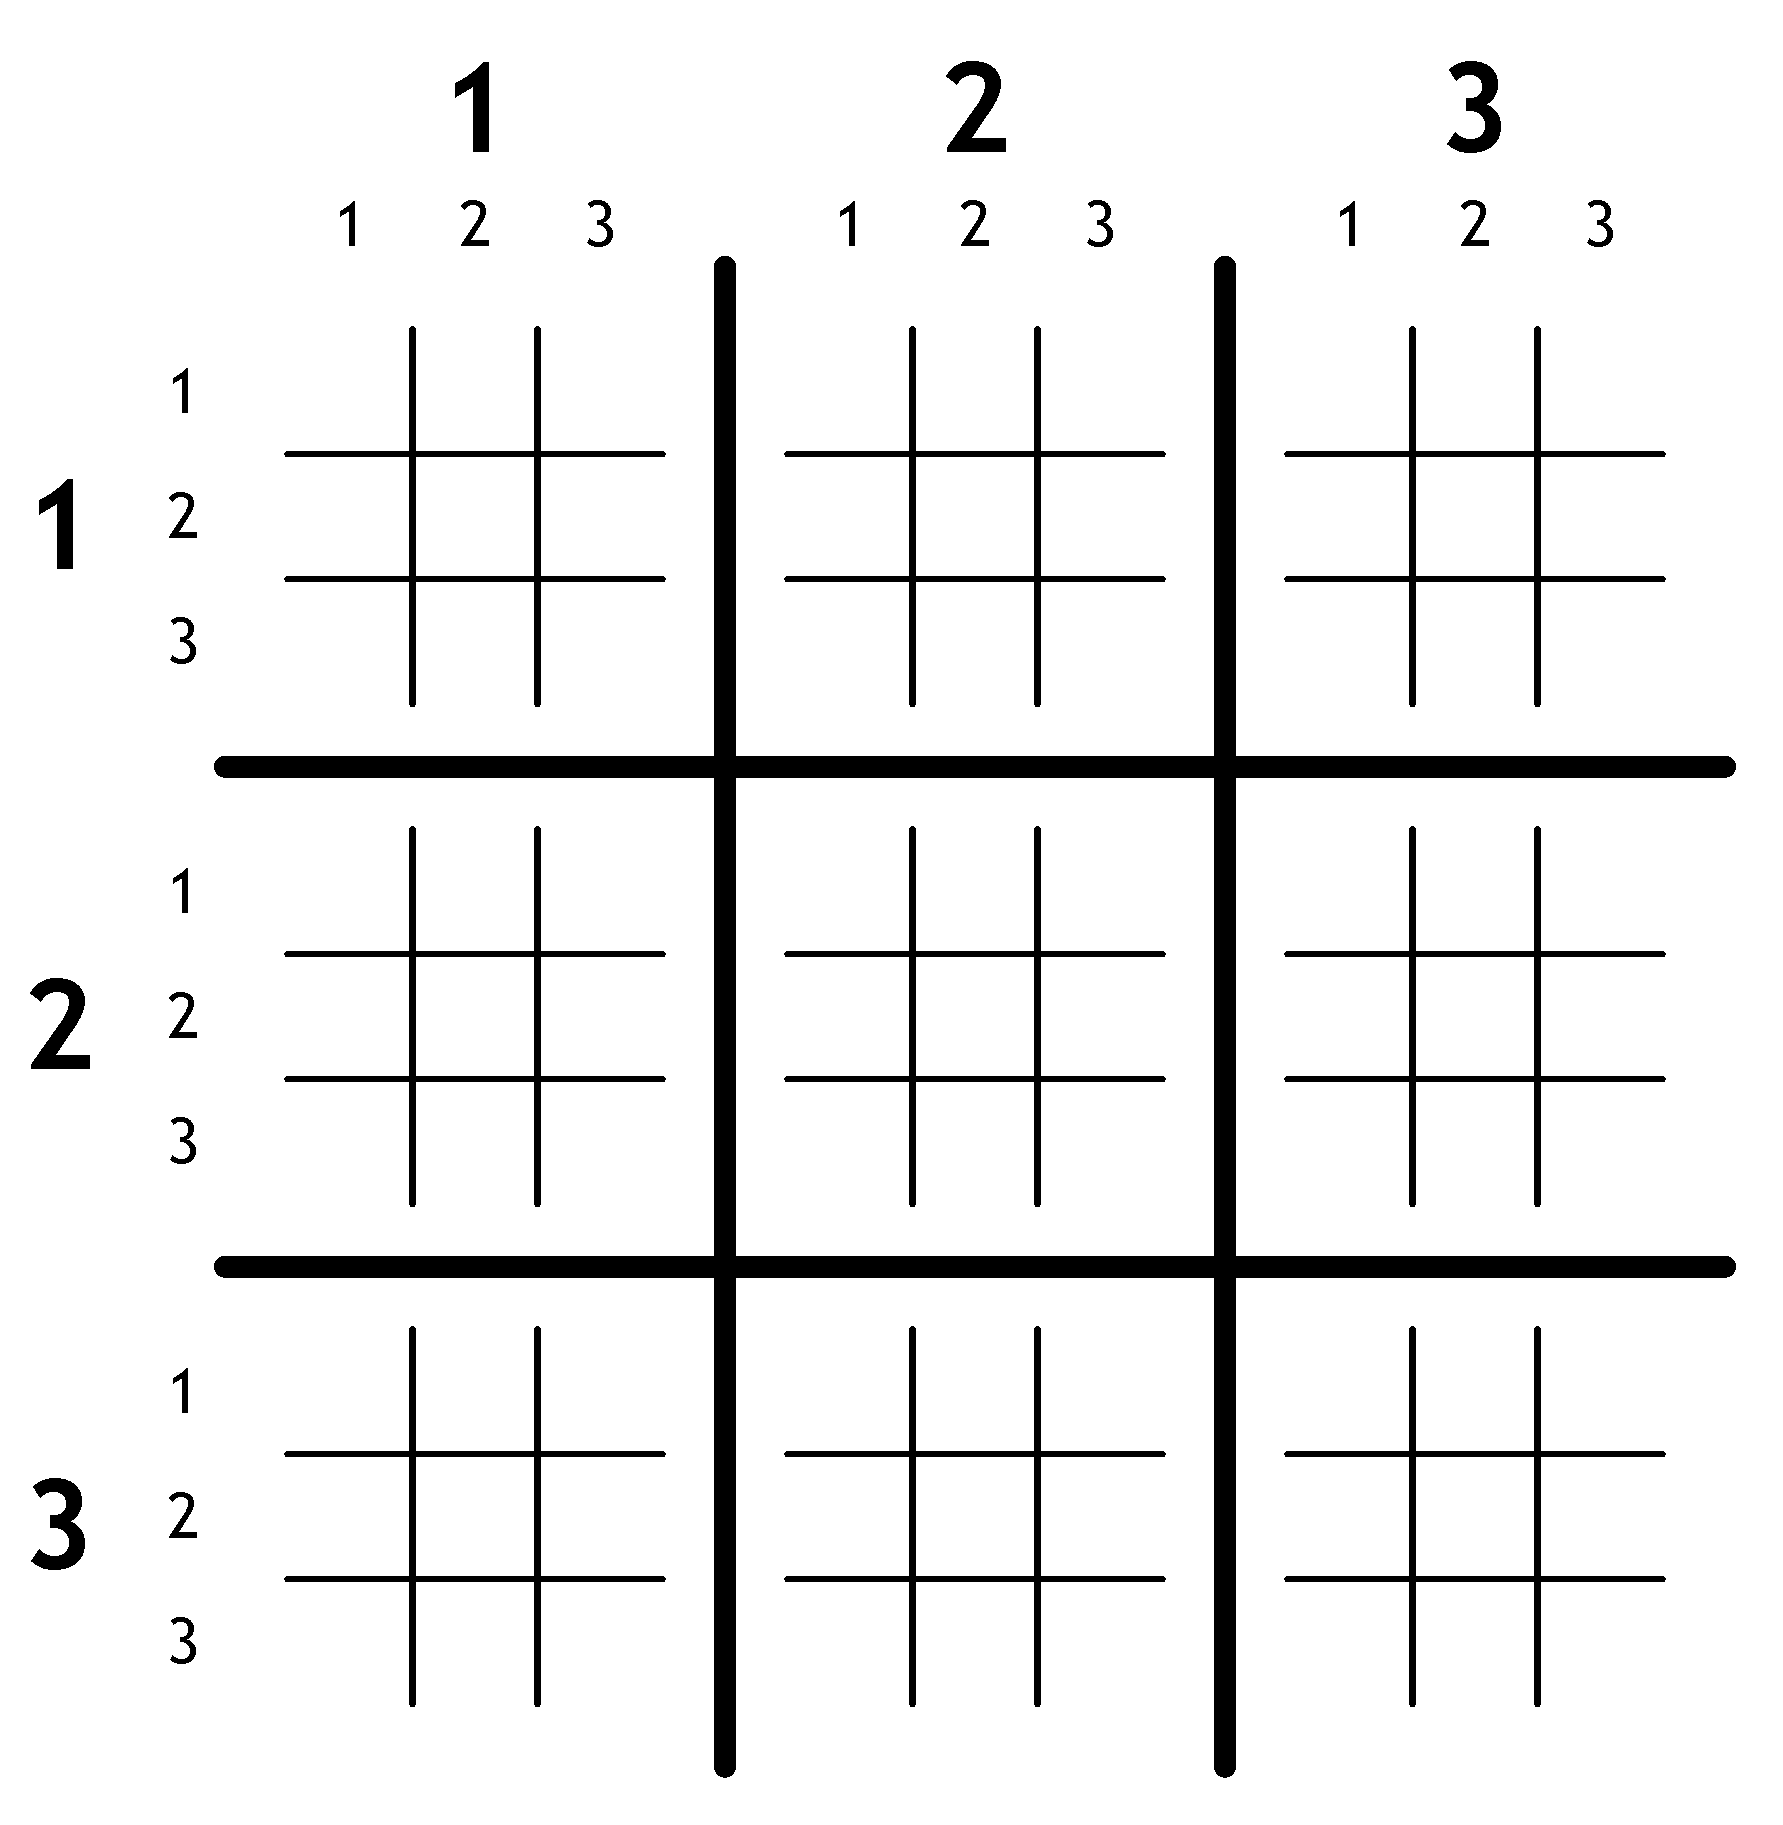
\includegraphics[width=0.7\linewidth]{diagram}
\end{center}

\subsection{Claiming}
Each tile can be uniquely identified by a [row, column] within the larger grid and a [row, column] within that smaller grid. For instance, the bottom left corner tile of the top right grid would be identified by the coordinates [1,3][3,1]. The center tile of the center grid is [2,2][2,2].

To claim a tile, a player first rolls 4 four-sided dice. They can then place one of their tokens to claim any unclaimed tile that can be identified by some permutation of their four dice (using the coordinate system mentioned previously). Rolling a 4 is a wildcard, and may be substituted for a 1, 2 or 3 at the player's discretion.

Players may not claim tiles that are already claimed, nor tiles that are within large tiles that are already claimed by either player. If a player is unable to claim any tile, then their turn is skipped.

\subsection{Tiebreakers}
When all 3-in-a-row possibilities are blocked within a single small grid, then the player with the most claimed tiles within that grid claims that tile in the large grid.

When every large tile has been claimed and neither player has 3-in-a-row in the large grid, then the player with the most claimed tiles in the large grid wins the game.

\section{Turn Example}
On their turn, the blue player rolls four dice that come up: 1, 2, 3, 3. With this roll, the player is able to claim one of the following tiles:

\begin{multicols}{3}
\begin{itemize}
\item {[}1,2][3,3]
\item {[}1,3][2,3]
\item {[}1,3][3,2]
\item {[}2,1][3,3]
\item {[}2,3][1,3]
\item {[}2,3][3,1]
\item {[}3,1][2,3]
\item {[}3,1][3,2]
\item {[}3,2][1,3]
\item {[}3,2][3,1]
\item {[}3,3][1,2]
\item {[}3,3][2,1]
\end{itemize}
\end{multicols}

\begin{center}
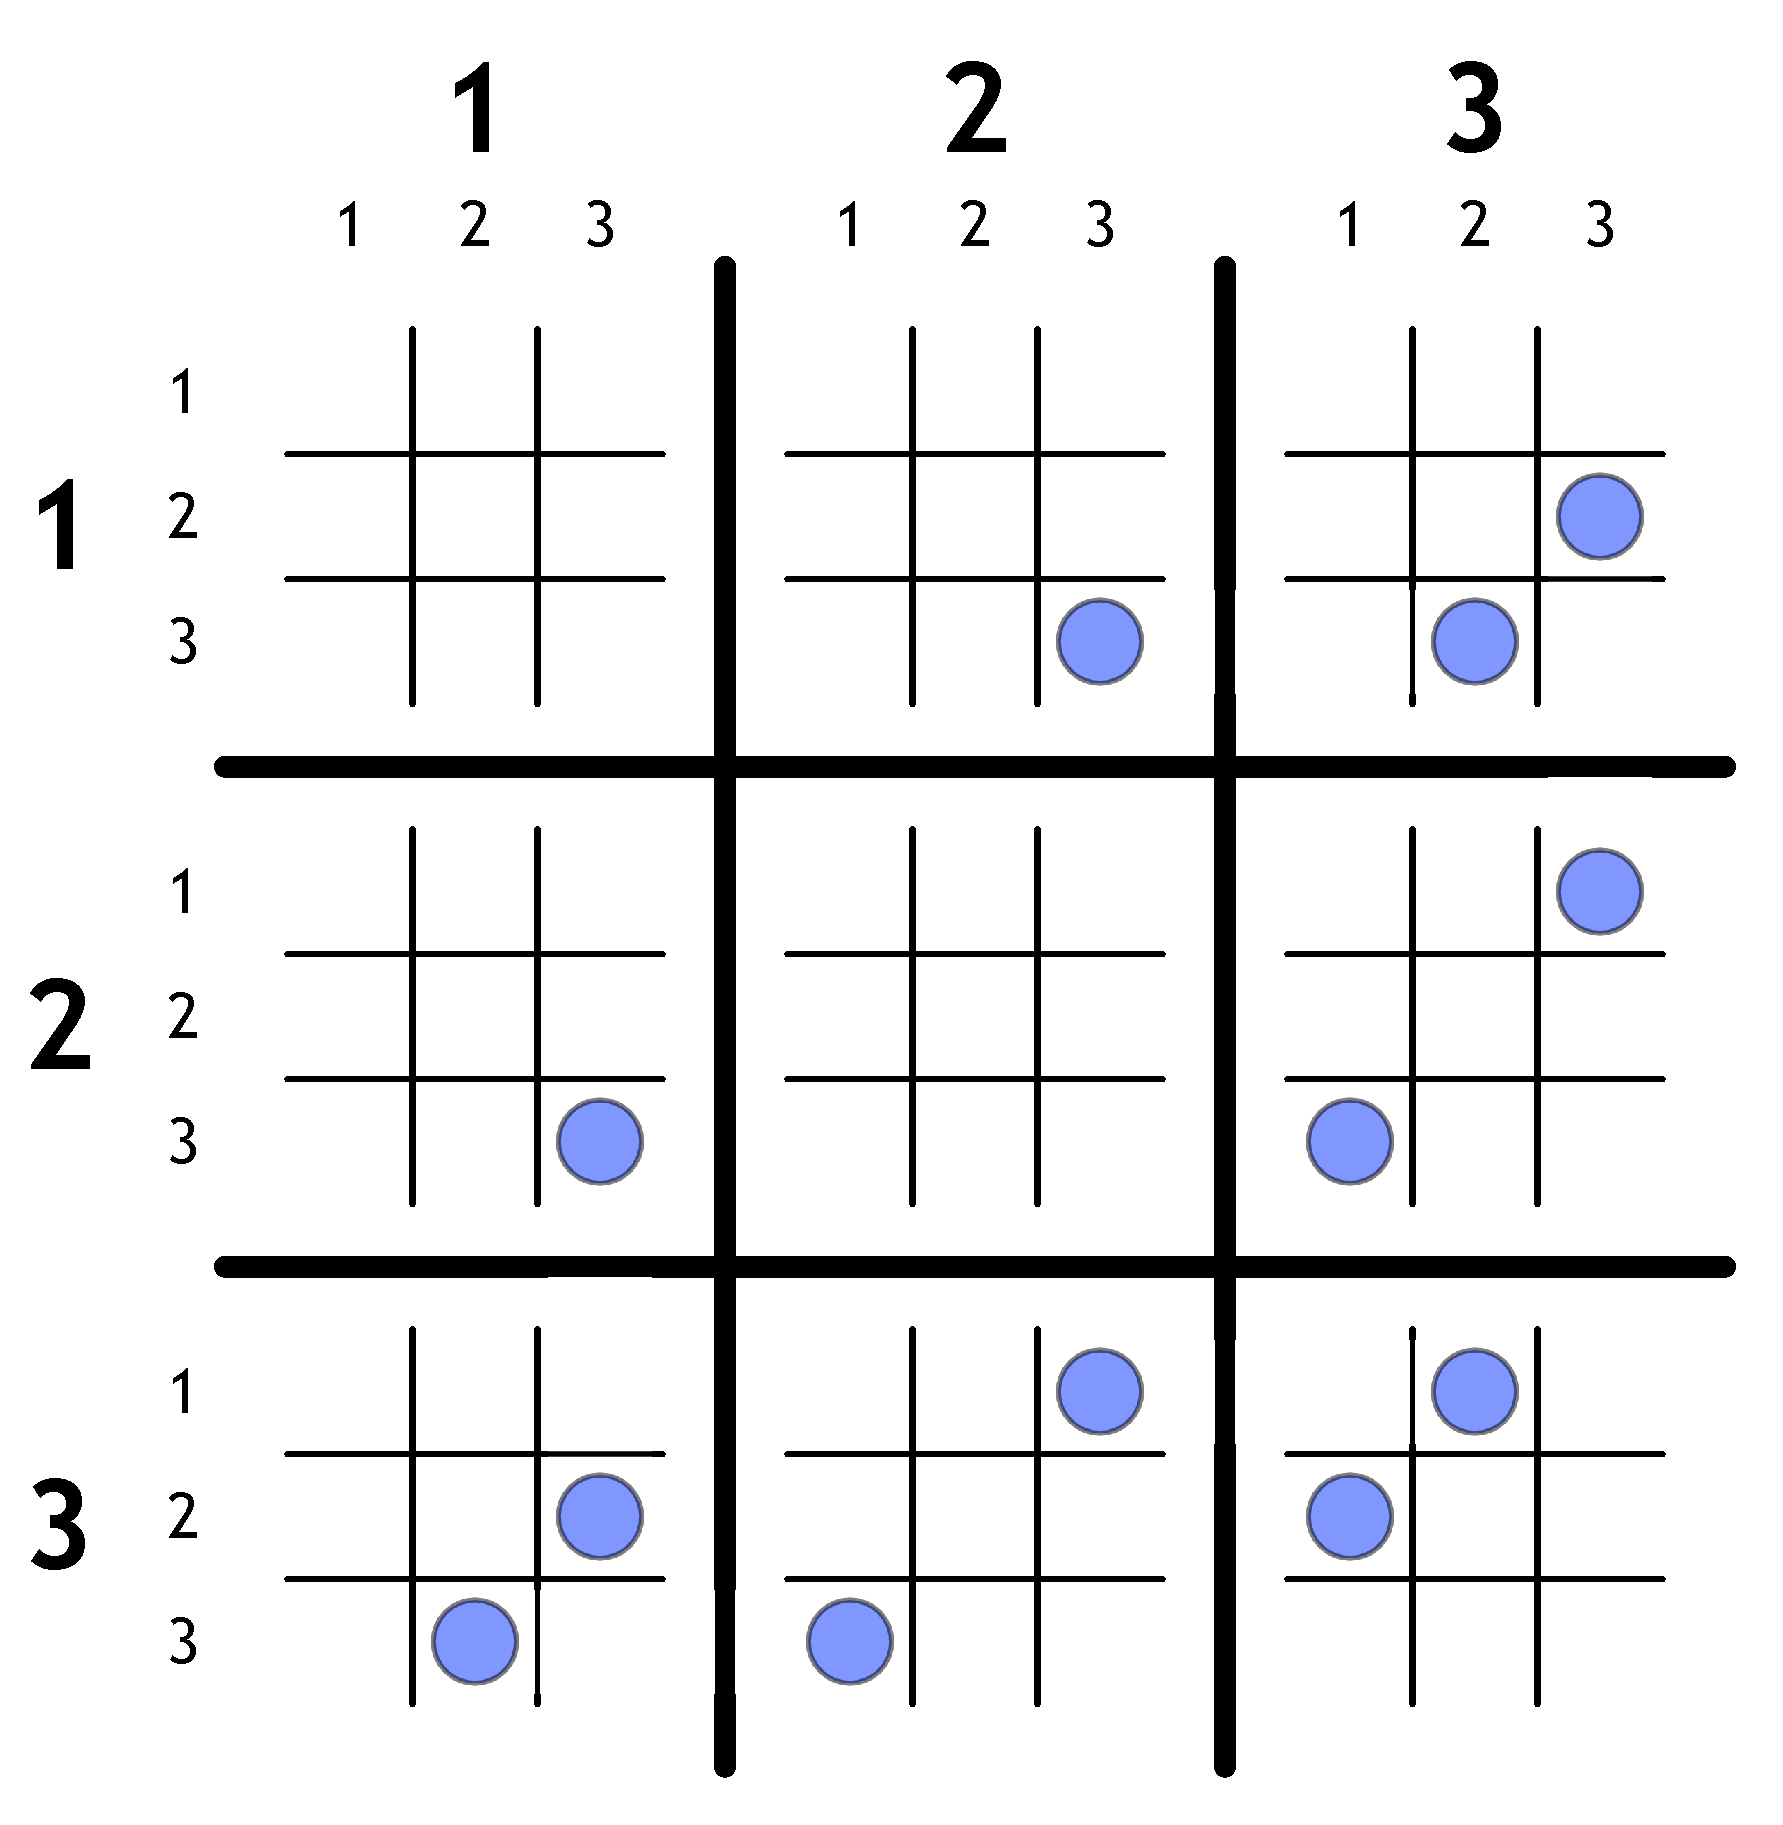
\includegraphics[width=0.8\linewidth]{diagram2}
\end{center}

\end{document}